% PACKAGES
\documentclass[a4paper, hidelinks, 12pt]{report}
\usepackage[margin=1in]{geometry}
\usepackage{amsfonts,amsmath,amssymb}
\usepackage[none]{hyphenat}
\usepackage{fancyhdr}
\usepackage{graphicx}
\usepackage[nottoc,notlot,notlof]{tocbibind}
\usepackage{hyperref}
\usepackage{longtable}
\usepackage[utf8]{inputenc}
\usepackage{multirow}
\usepackage{booktabs}
\usepackage[font=footnotesize]{caption}
\usepackage[flushleft]{threeparttable}
\usepackage{relsize}
\usepackage[super,negative]{nth}
\usepackage{enumerate}
\usepackage{float}

\usepackage[dvipsnames]{xcolor}
\usepackage{listings}
\usepackage[T1]{fontenc}
%\usepackage{alloy-style}
%%%%%%%%%%%%
% DOC STYLES
%\makeatletter
\def\thickhrulefill{\leavevmode \leaders \hrule height 1ex \hfill \kern \z@}
\def\@makechapterhead#1{
	\vspace*{4\p@}
	{\parindent \z@ \centering \reset@font
		\thickhrulefill\quad
		\scshape \@chapapp{} \thechapter
		\quad \thickhrulefill
		\par\nobreak
		\vspace*{4\p@}
		\interlinepenalty\@M
		\hrule
		\vspace*{4\p@}
		\Huge \bfseries #1\par\nobreak
		\vspace*{4\p@}
		\hrule
		\vskip 50\p@
}}
\def\@makeschapterhead#1{
	\vspace*{4\p@}
	{\parindent \z@ \centering \reset@font
		\thickhrulefill
		\par\nobreak
		\vspace*{4\p@}
		\interlinepenalty\@M
		\hrule
		\vspace*{4\p@}
		\Huge \bfseries #1\par\nobreak
		\vspace*{4\p@}
		\hrule
		\vskip 50\p@
}}

\pagestyle{fancy}
\fancyhead{}
\fancyfoot{}
\fancyhead[L]{\slshape\MakeUppercase{\textbf{RASD}}}
\fancyhead[R]{\slshape{Morreale,Maddes,Innocente}}
\fancyfoot[C]{\thepage}
\renewcommand{\footrulewidth}{1pt}
\renewcommand{\headrulewidth}{1pt}
\linespread{1.3}
%\floatstyle{boxed}
\restylefloat{figure}
\parindent 0ex
%\renewcommand{baselinestretch}{1.5}

%%%%%%%%%%%%

% COMMANDS
\newcommand\requirement[1]{\item[{[R#1]}] }
\newcommand\goal[1]{\item[{[G#1]}] }
\newcommand\assumption[1]{\item[{[D#1]}] }
\newcommand\usecase[1]{ [UC#1] }

%%%%%%%%%%%%

%BODY
\begin{document}
	\begin{titlepage}
		\centering
		\vspace*{0.7 cm}
		
\includegraphics[scale = 0.85]{assets/polimi.png}\\[1.6 cm]
		\textsc{\large Department of Computer Science and Engineering}\\[1.8 cm]

		\rule{\linewidth}{0.2 mm} \\[0.4 cm]
		{ \huge \bfseries Requirement Analysis and Specification Document (RASD)}\\
		\rule{\linewidth}{0.2 mm} \\[1.5 cm]

		\textsc{\Large Safe Streets}\\[0.5 cm]
		\textsc{\large - v1.0 -}\\[1 cm]

		\begin{minipage}{0.4\textwidth}
			\begin{flushleft} \large
				\emph{Authors:}\\
				\textbf{Morreale} Federico \\
				\textbf{Maddes} Evandro \\
				\textbf{Innocente} Federico
			\end{flushleft}
		\end{minipage}~
		\begin{minipage}{0.4\textwidth}
			\begin{flushright} \large
				\emph{Student Number:} \\
				945238 \\
				945642 \\
				000000
			\end{flushright}
		\end{minipage}\\[2 cm]

		{\large November \nth{10} , 2019}\\[2 cm]

		\vfill
	\end{titlepage}

	\pagenumbering{roman}
	\tableofcontents
%	\thispagestyle{empty}
	\newpage
	%\listoffigures
	%\listoftables
%	\thispagestyle{empty}
	\clearpage
	\pagenumbering{arabic}
	\setcounter{page}{1}

	\chapter{Introduction}\label{ch:introduction}
	\section{Purpose}\label{sec:purpose}
        \subsection{General Purpose}\label{subsec:general-purpose}
            The purpose of the Requirement Analysis and Specification Document (RASD) is to give a clear and non-ambiguos analysis of SafeStreet, an application that will be implemented, describing every aspects of it like functional/non-functional requirements, constraints, domain assumptions, providing use cases and scenerios of the external world. Moreover, a more formal analysis of some relevant functions of the system will be provided using Alloy, a declarative specification language for expressing complex structural constraints and behavior in a software system.
            SafeStreets is a crowd-sourced application that intends to provide users with the possibility to notify authorities when traffic violations occur, and in particular parking violations.
            \begin{itemize}
                \item \textbf{Basic Service:}
                it allows every user to take a picture of a violation with a brief description and send everything, including date,time, position and license plate, to SafeStreet, that will give access to all the information, with different levels of visiblity, to both citizens and police officers. In addition to that, Safestreet will provide the areas with the highest number of violations and a ranking of the vehicles that commit the major number of infractions.
                \item \textbf{Advanced Function 1:}
                it allows SafeStreet to cross information about accidents that occur on the territory of the municipality with its own, in order to give useful advices by suggesting possible interventions. This service is possible if, and only if the local municipality shares its data to SafeStreet.
                \item \textbf{Advanced Function 2:}
                it allows the municipality to generate traffic tickets from the data stored in SafeStreet, of course that data has to be previously validated by the system, preventing malicious corruptions by offenders. Moreover, having the information about issued tickets, SafeStreet can build statistics and share them among all users.
            \end{itemize}
        \subsection{Goals}\label{subsec:goals}
            SafeStreet is a service provided to people to notify both other people and authorities about traffic violations. There are two different classes of users to whom the software is addressed: standard users and authorities, which have two different ways to interact with the application.
            In order to perform correctly, the software-to-be will have to grant that some services will be guaranteed. Below is given a list of all the goal of the software-to-be:
            \begin{enumerate}
                \goal{1} The application will allow users to upload pictures of the traffic violations, with the possibility of adding as information the date, time, position, type of infringement and a textual description.
                \goal{2} The application will allow users to query the information about the violation, to know which kind of violations have been done in an area defined by the users.
                \goal{3} The application will allow only the authorities to see the pictures uploaded by the users.
                \goal{4} The application won’t give any information to the standard users about the people involved into violation, in order to grant their privacy.
                \goal{5} If SafeStreets can get the information about accidents by the municipality, it will give the possibility to merge them with its data to identify potentially unsafe areas.
                \goal{6} If SafeStreets can get the information about accidents by the municipality, it will give the possibility to merge them with its data to suggest possible interventions.
                \goal{7} The system will use the information about violations, accidents and fines that will collect by both users and authorities to build statistics.
                \goal{8} Users can give a feedback about violations uploaded by other users to SS.
            \end{enumerate}
	\section{Scope}\label{sec:scope}
        \subsection{World, Machine and Shared phenomena}\label{subsec:world,-machine-and-shared-phenomena}
            According to \textit{The World and the Machine} we can divide every system into two parts:
            \begin{itemize}
                \item The \textbf{machine}, which is the portion of system to be developed;
                \item The \textbf{world}, which is the portion of the real-world affected by the machine.
            \end{itemize}
            As a consequence we can classify phenomena in three different types:
            \begin{itemize}
                \item \textbf{World phenomena}: phenomena that the machine cannot observe;
                \item \textbf{Machine phenomena}: phenomena located entirely in the machine;
                \item \textbf{Shared phenomena}: phenomena that can be controlled by the world and observed by the machine or controlled by the machine and observed by the world;
            \end{itemize}
            Below we give an analysis of the three phenomenas descripted above:
            \begin{itemize}
                \item \textbf{World Phenomena}
                \begin{itemize}
                    \item Users recognize the type of violation that occurred
                    \item People commit violations
                    \item People perform incidents
                    \item Police emit traffic tickets
                \end{itemize}
                \item \textbf{Machine Phenomena}
                \begin{itemize}
                    \item Machine manages database queries;
                    \item Machine stores information (picture with other data or only data) on the database;
                    \item Machine runs an algorithm periodically to builds statistics (veichels with most number of violation or trends in the issuing tickets );
                    \item Machine runs an algorithm periodically to identify potentially unsafe areas;
                    \item Machine manages interfaces with external software (for recognition of a text from an image) and hardware system (for take a picture).
                \end{itemize}
                \item \textbf{Shared Phenomena}
                \begin{itemize}
                    \item Users have to take and upload the pictures of the violations;
                    \item Users and authorities query the system about violations;
                    \item The machine gets the information about the accidents by the local municipality;
                    \item The machine use report about violations and accidents to the local municipality to submit possible solution, that can be both considered or not;
                    \item The municipality can mark reported violations as fined, to allow the system to perform statistics about effectiveness of SafeStreet.
                \end{itemize}
            \end{itemize}

	\section{Definitions, Acronyms, Abbreviations}\label{sec:definitions,-acronyms,-abbreviations}
        \subsection{Definitions}\label{subsec:definitions}
            \begin{itemize}
                \item \textbf{User:} is a general customer that use the application. It is used to refer to both an authority and a ciziten.
                \item \textbf{Citizen:} is the basic customer of the application. He can upload violations and query the system to get statistics on a selected area.
                \item \textbf{Authority:} advanced customer of the application, is a registered user that is qualified to make fines. Must verify himself during the registration.
                \item \textbf{Municipality:} is always intended as the local municipality. Every municipality provide and receives information exactly and only about its own jurisdiction.
                \item \textbf{Violation:} is a general infringement reported by a user.
            \end{itemize}

        \subsection{Acronyms}\label{subsec:acronyms}
            \begin{itemize}
                \item RASD: Requirement Analysis and Specification Document
                \item SS: SafeStreets
                \item LP: License Plate
                \item GPS: Global Positioning System
                \item API: Application Programming Interface
                \item UML: Unified Modeling Language
            \end{itemize}

        \subsection{Abbreviations}\label{subsec:abbreviations}
            \begin{itemize}
                \item $[Gn]$: n-goal.
                \item $[Dn]$: n-domain assumption.
                \item $[Rn]$: n-functional requirement.
                \item $[UCn]$: n-use case.
            \end{itemize}

	\section{Reference Documents}\label{sec:reference-documents}
        This document follows ISO/IEC/IEEE 29148:2011 and IEEE 830:1998  standard for software product specifications.
        All the specifications of this project have been given by Rossi and Di Nitto for the Software Engineering 2 Mandatory Project 2019-2020.

	\section{Revision history}\label{sec:revision-history}
	.

	\section{Document structure}\label{sec:document-structure}
        \textbf{Chapter 1: Introduction.} A general introduction to the goals, the phenomena and the scope of the system-to-be. It aims giving general but exaustive informations about what this document is going to explain.
        \\
        \textbf{Chapter 2: Overall description.} A general description of the product to be and its requirements. This section provides several information that are detailed explained in Section 3.
        \\
        \textbf{Chapter 3: Specific requirements.} All software requirements are explained using scenarios, use-case diagram and activity diagram. Non-functional and functional requirements are also cited.
        \\
        \textbf{Chapter 4: Alloy.} This section includes Alloy code that describes the model and checks whether it is consistent or not.
        \\
        \textbf{Chapter 5: Effort Spent.} A summary of the worked time by each member of the group.

	\chapter{Overall description}\label{ch:overall-description}
	    \section{Product perspective}\label{sec:product-perspective}
	    In the previous section, the scope of the application was delimited and explained in a shallow way, but at this point it is useful to include further details on the shared phenomena and a domain model as a visual representation of the system.
    \begin{center}
    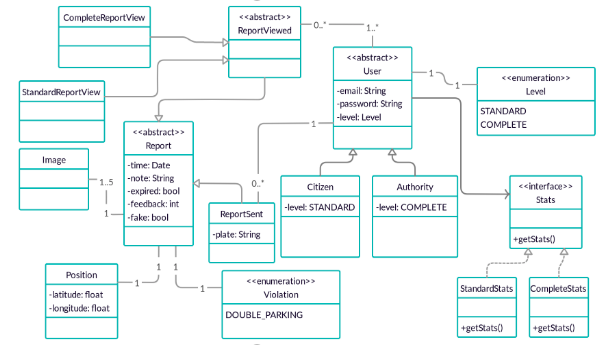
\includegraphics[scale = 0.85]{assets/domainModel.png}\\[1.6 cm]
    \end{center}

    Generic violation report:

	    To understand the main events happening in the system, it is useful to use statechart diagrams (described in the figure below). At the beginning each report(i.e. when a user uploads an image) is considered as unprocessed. While the constraints are checked (there must be: at least one photo, the type of violation, and if it’s a car violation the license plate is mandatory too as a picture), the report is on a pending state and can become either rejected or approved. In the end, it’s considered completed and the user is notified with the outcome. If it’s been approved, the report is kept in the database.

    \begin{center}
        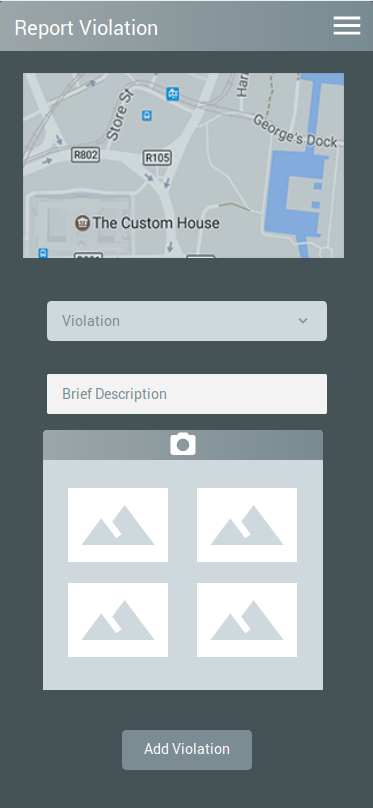
\includegraphics[]{assets/report.png}\\[1.6 cm]
    \end{center}

	    Query to database:

    	In case there is a query for get information about one selected violation, it can be made by a citizen or by an authority and this establishes different results showed by the system: in the former case SafeStreets returns information and photos about selected violation but doesn’t show photos about license plate for privacy reason (system must guarantee anonymity) instead in the latter case SafeStreets returns all the photos and other information about violation so authority can use them to generate traffic tickets.

    \begin{center}
        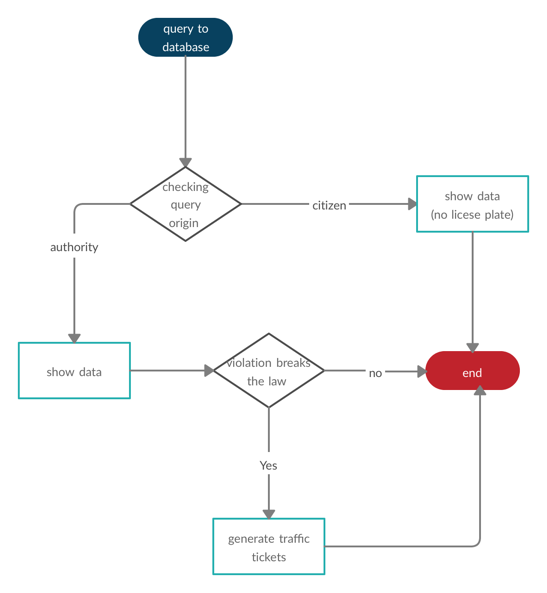
\includegraphics[]{assets/queryDb.png}\\[1.6 cm]
    \end{center}

	    Build statistics:

	    When one authority uses violation taken from SafeStreets, he marks the violation as fined.

	    Authorities can also upload accidents on the through a dedicated interface.

	    The system periodically distinguishes violations that are used by authorities from the others so can builds statistics on the effectiveness of the application. It also analyzes, querying the database, the different type of the violation and the vehicles involved. This informations are both used to build statistics and to find unsafe area(also using data about accidents), in the last case system provide a suggestion for the problem.

    \begin{center}
        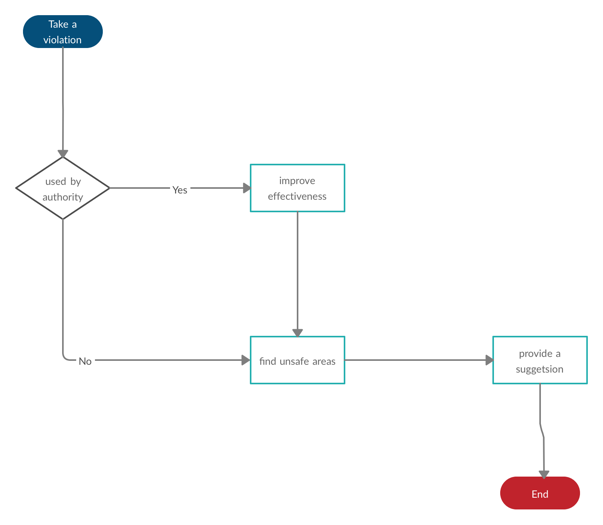
\includegraphics[]{assets/buildStatistics.png}\\[1.6 cm]
    \end{center}
        \section{Product functions}\label{sec:product-functions}
         In the following we will present the main aspects and functions of the system, to put in evidence the most important requirements that will be formalized in chapter 3.
    \subsection{Citizens functions}\label{subsec:citizen-functions}
    A person can register himself to the SafeStreet system by providing a valid email address and a password. No other data will be mandatorily required, but the user will be allowed to set a residential location to personalize the user interface.

    Every registered user that see a traffic violation can report it throw SafeStreet: to do that, he has to upload at least one picture of the infringement and provide some information about it. The user can upload at least one pictures of the environment to show the violation, but those can be only taken by a specific tool of the application that won't allow to modify the photos. This restriction is applicate to not let people to upload pictures that could have been modified to accuse someone extraneous to the burglary. The user will have to add to the images the position (that will be possible to be taken throw the device GPS) and will have to indicate the category of the violation as mandatory information, while will be able to add a text description to possibly give more information.

    Every user will be arable to consults a map that will show all the reported violations of the last 24 hours. Citizens will even be allowed to query the application about the violations reported by the community. To do that, he will have to define one or more constrains between a marked zone on a map, a time frame and a specific category, to get all the correspondent infringement reported, respectively, in that zone, period or category. When a user will look for a violation, he will be able to see all the information uploaded for it, except for the vehicle target plates, that will be obscured because of privacy reasons.

    Every user will be allowed to report a violation uploaded by another user that don’t subsists, because of the description or the pictures don’t match with each other. When a violation has been reported by five different people is removed from the system and no more available. In the same way, a user can report one of the photos of the violation because of an affection of the privacy of another person (for instance if a license plate is visible). After five report from different people, the picture will be deleted from the dossier if at least one other picture is available; otherwise, the whole violations will be removed by the system.
    \subsection{Authority functions}\label{subsec:authority-functions}
    To register as an authority, a person has to be part of the national police force. To accede to the application, he has to register by entering an email address and a password that he will use to sing in, and his freshman to certificate himself. An authority can access both all the functionality of a citizen and some advanced ones.

    When an authority queries the system to get the violations, SafeStreet will show him all the information about the report, including the uncensored pictures uploaded by the users. This is done in order to give to the authority the possibility to fine whoever committed the crime if they are able to track him down. An authority can mark the dossier of a violation that he fined to let all the users know that it has been sanctioned. Users can query the system to get all the sanctioned violations, to have a feedback about which kind of infringement or information are more likely to be sanctioned.
    \subsection{Municipality featuring functions}\label{subsec:municipality-featuring-functions}
    Every local municipality can join into SafeStreet by identifying itself throw his own national identifier. Once the registration has been confirmed, the system will provide a dedicate page to manage the collaboration between SafeStreet and the municipality.

    If the municipality provide information about the accidents that occurs in its territory, SafeStreet can collect them to cross them with the reported violations. If the system can find a correlation between the violations and the accident it can mark a map of the most unsafe areas, identifying them with a higher level of dangerous with the increasing number of accidents. The system will also be able to verify the typology of the violations that have been reported by the user in the area that concern every accident, to provide an ad hoc solution to cope the most frequent class of violation, if this has been registered a significant number of times.
    \section{User characteristics}\label{sec:user-characteristics}
    The target users of the SafeStreets system are:
    \begin{itemize}
        \item \textbf{Citizens:}
        \begin{itemize}
            \item Can register and then login to the app ;
            \item Can upload violations ;
            \item Can get all the violations uploaded by the other users ;
            \item Can check the presence of unsafe areas;
        \end{itemize}
        \item \textbf{Authorities:}
        \begin{itemize}
            \item Can register and then login to the app using their IDs to acknowledge  ;
            \item Can upload violations ;
            \item Can get all the violations uploaded by the other users ;
            \item Can check the presence of unsafe areas;
            \item Can get the list of the worst offenders in the city;
            \item Can generate traffic tickets after checking the violation on the app;
        \end{itemize}
    \end{itemize}
    \section{Assumptions, dependencies and constraints}\label{sec:assumptions,-dependencies-and-constraints}
            \subsection{Domain assumptions}\label{subsec:domain-assumpiton}
                \begin{enumerate}
                    \assumption{1} GPS position collected when the report is being uploaded is sufficiently accurate.
                    \assumption{2}SS guarantees very strong data protection and integrity against malicious external attacks.
                    \assumption{3} The map that shows all the current violations represent the topology of the city.
                    \assumption{4} License plates attached to the cars are legit.
                \end{enumerate}
            \subsection{Dependencies}\label{subsec:dependencies}
            \begin{itemize}
                \item Traffic tickets can be emitted only if the user upload the picture of the violation with the license plate visible and recognizable by the authorities.
                \item Users must input the right violation according to what they are reporting, otherwise statistics may be inaccurate.
                \item Current date and time of a report are taken by SS from its local clock as soon as it is being uploaded, that is synchronized according UTC.
            \end{itemize}
            \subsection{Constraints}\label{subsec:constraints}
            \begin{itemize}
                \item Smartphones must have GPS and be activated when uploading a violation.
                \item Smartphones must have internet connection turned on (WIFI or 3G/4G) while using the app.
                \item Users must accept the privacy policy in order to use the application.
                \item Smartphones must have at least 100Mb of available memory in order to install the app
                \item Smartphones must have at least 1Gb RAM in order to run the application.
                \item Smartphones must have a camera in order to upload violations.
                \item Users must have a personal email address in order to sign up and therefore use the app.
            \end{itemize}
    \chapter{Specific requirements}\label{ch:specific-requirements}
    This section contains all of the functional and quality requirements of the system. It gives a detailed description of the system and all its features.
    \section{External interface requirements}\label{sec:external-interface-requirements}
        \subsection{User Interfaces}\label{subsec:user-interfaces}
        \subsection{Hardware Interfaces}\label{subsec:hardware-interfaces}
        \subsection{Software Interfaces}\label{subsec:software-interfaces}
        \subsection{Communication Interfaces}\label{subsec:communication-interface}
    \section{Functional requirements}\label{sec:functional-requirements}
        \subsection{Scenarios}\label{subsec:scenarios}
        \subsection{Use case diagram}\label{subsec:Use-case-diagram}
    \section{Performance requirements}\label{sec:performance-requirements}
    \section{Design constraints}\label{sec:design-constraints}
        \subsection{Standard compliance}\label{subsec:standard-compliance}
        \subsection{Hardware limitations}\label{subsec:hardware-limitations}
        \subsection{Any other constraints}\label{subsec:any-other-constraints}
    \section{Software system attributes}\label{sec:software-system-attributes}
        \subsection{Reliability}\label{subsec:reliability}
        \subsection{Availability}\label{subsec:availability}
        \subsection{Security}\label{subsec:security}
        \subsection{Maintainability}\label{subsec:maintainability}
        \subsection{Portability}\label{subsec:portability}


\end{document}
